\subsection{Cloud Reference Architectures for Industrial IoT}
\label{subsection:cloud-ref}
    In this section, we will examine the reference architectures for IIoT as designed by major cloud providers such as Microsoft Azure, Amazon Web Services, and Google Cloud Platform. Our focus will be on identifying their limitations and exploring why they may not entirely meet the evolving requirements of contemporary IIoT systems thus emphasizing the need for a modern reference architecture in this sector. \newline 

    % \subsubsection{Structure of cloud reference architectures}

    One of the most common design frameworks used for IIoT scenarios is the ``Microsoft Azure IoT Reference Architecture''. The framework is targeted to IoT in general and will be refined towards IIoT later with the ``Microsoft Azure Industrial Internet of Things''. The reference architectures of other cloud providers are often similar and only differ in details, which will be mentioned later. 
    
    \autoref{figure:azure-reference} shows a high-level overview of the architecture in question. Similar to what was recommended in the IIRA in \autoref{subsubsection:iira} the structure is separated into three tiers, where each tier has its own responsibilities. The architecture describes four kinds of components within the system: devices, a cloud gateway service, stream processors and a user interface. Devices and/or on-premise edge gateways are responsible for registering (often referred to as onboarding) within the cloud system and having connectivity options with the cloud for sending and receiving data. 
    
    \begin{figure}[htbp]
        \centering
        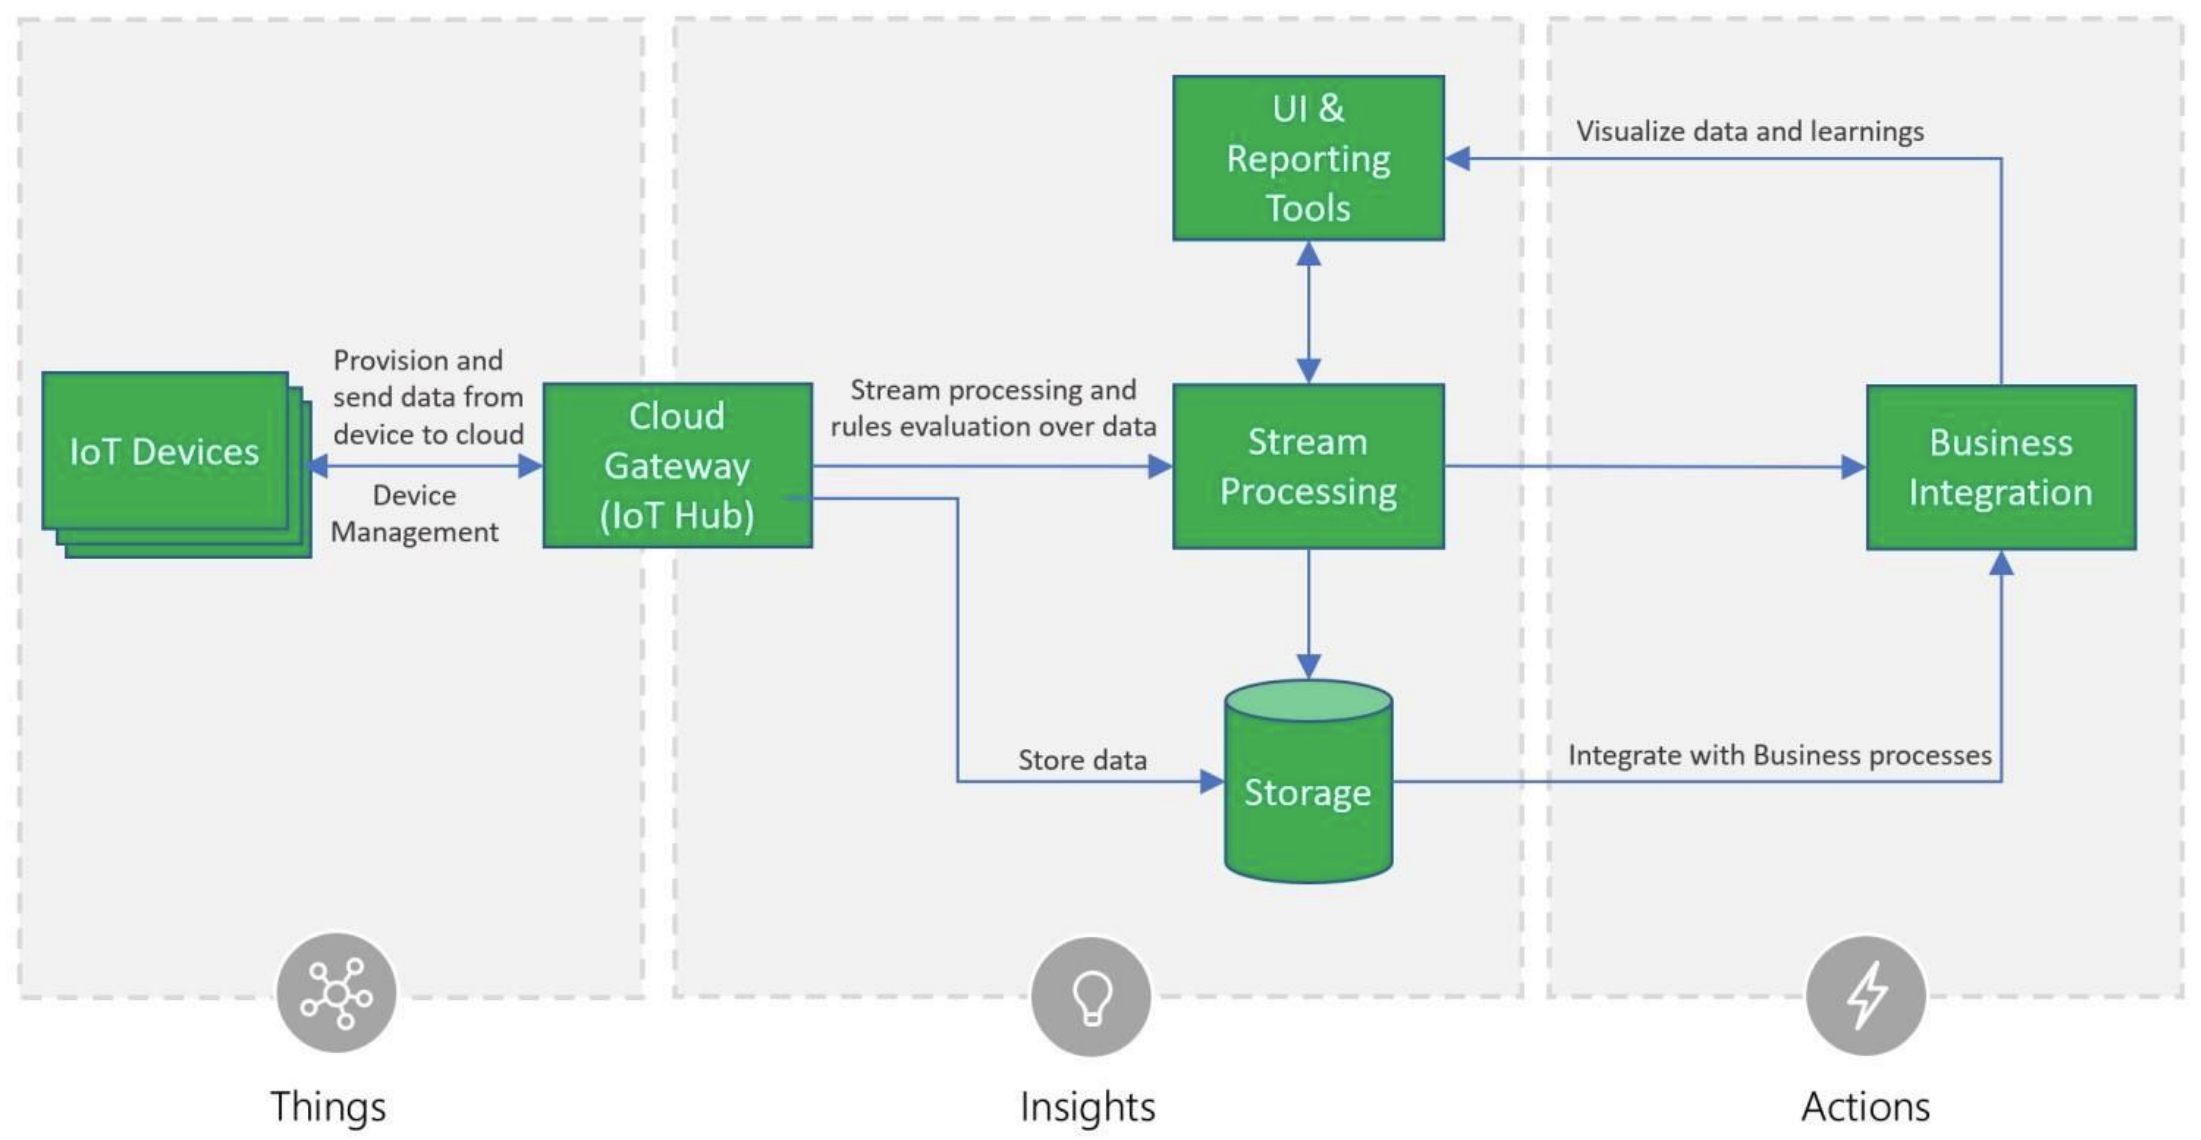
\includegraphics[width=0.9\textwidth]{img/azure-reference.png}
        \caption{Microsoft Azure IoT Reference Architecture: Overview \cite{microsoft_azure_iot_reference}}
        \label{figure:azure-reference}
    \end{figure}
    
    \noindent The receiver of this data is a cloud gateway service, also known as a hub. Its tasks include device management and securely communicating with both upstream and downstream components, while most importantly acting as the bridge to the cloud. Here we can see the main architectural difference to the three-tier architecture described in the IIRA in \autoref{subsubsection:iira}, which is, that all data is sent directly from the devices to the cloud for further processing, whereas in the IIRA, the ``platform tier'' might also be built on-premises. From here on managed cloud services can be used which is a major benefit when dealing with big data, since a large amount of processing power, storage and network bandwidth is available. Stream processors are components that consume data, integrate with business processes and place data into storage. Lastly, a user interface is required to visualize telemetry data and facilitate device management. Apart from the system architecture itself, the Azure IoT reference architecture also deals with other concerns, mainly managed cloud resources. Since we will later see that the reference architecture is not sufficient for many use cases, and managed resources are very cloud provider-specific, this is out of the scope of this work. \newline
    
    Diving deeper, one of the main components used in the Azure IoT architecture is the ``Azure IoT Hub''. It acts as the cloud gateway service and is a managed, highly scalable service that acts as a central message hub for communication. It behaves similarly to an MQTT broker (see \autoref{subsubsection:mqtt}) but apart from MQTT also supports data transfer with the protocols ``Advanced Message Queuing Protocol (AMQP)'' and HTTPS. It also integrates nicely with other cloud services by Azure, like Azure Event Grid for reacting to events, Azure Machine Learning for implementing AI solutions or Azure Stream Analytics for real-time analytic computations. Since it runs in the cloud, it's possible to subscribe and react to events on the factory floor from anywhere in the world. However while typical IoT devices like smart home devices can easily run software that can communicate using protocols like MQTT, this is often not possible in IIoT due to reasons like resource or network constraints as discussed in \autoref{section:current-situation} \cite{microsoft_azure_iot_reference}.
    
    For applying this architecture to industrial IoT scenarios, Microsoft Azure provides guidance with the ``Microsoft Azure Industrial Internet of Things''. It is described as a suite of Azure cloud microservices and Azure IoT Edge modules and is said to provide the ability to integrate data from assets, sensors and existing systems into the Azure cloud using protocols like OPC-UA which was discussed in \autoref{subsection:opc-ua}. A system following this architecture is constructed of at least one Azure IoT Hub, one or more Azure IoT Edge devices and various Azure IoT Edge modules. The IoT Hub, which has been previously described, acts as the central communication node and thus requires no further explanation. An Azure IoT Edge device is again composed of two components, namely an edge device and edge modules. The edge device itself is physical hardware running the software Azure IoT Edge on top of Linux or Windows, which can be described as a runtime that enables cloud functionality to be extended to local or edge devices. It allows developers to deploy, run and monitor containerized Linux workloads, which follows the same idea as orchestration tools discussed in \autoref{section:orchestration-scheduling}. Devices with this runtime can be remotely monitored and managed through a cloud-based interface. On this runtime, so-called ``IoT Edge modules'', which represent units of execution, implemented as Docker-compatible containers, that run business logic at the edge, are deployed. While Azure provides prebuilt modules, custom ones can be built and deployed as well, which helps with fulfilling the requirement of running workloads at the edge as analyzed in \autoref{section:edge-computing}. 
    
    An example use case for an edge module is the preprocessing and compression of data, since sending raw sensor readings across the communication link to the cloud is not desirable, especially in network-constrained scenarios. Note that these IoT edge devices don't necessarily have to be where the data is actually created. Actual components like sensors that might communicate using protocols like S7 or even OPC-UA (\autoref{subsection:opc-ua}) can send their data to the IoT edge device, where protocol adapters, which are deployed as containerized applications, can then handle the translation to a protocol supported by the receiving Azure IoT Hub. This shows, that the reference architectures by cloud providers as expected often focus on the cloud side while neglecting the on-premises side which often requires other strategies like using OPC-UA \cite{microsoft_azure_iot_reference} \cite{iot_edge_docs} \cite{azure_iiot_overview}.

    As mentioned at the beginning of this section, IIoT reference architectures of other big cloud providers are of very similar structure. The solution of Amazon Web Services (AWS) for example uses ``AWS IoT Core'' as its cloud gateway instead of the Azure IoT Hub and ``AWS Greengrass'' as its edge runtime as a substitute for Azure IoT Edge, where both are very similar to their counterparts. AWS' IIoT solutions have a small advantage over the Azure solutions when it comes to flexibility since they support uncontainerized workloads and any kind of programming language whereas Azure IoT solutions only support containerized workloads written in a specified set of languages. This advantage is however irrelevant when it comes to the shortcomings of the reference architectures \cite{greengrass_vs_iot_edge}. Much alike is the IoT solution of Google called ``Google IoT Core''. Here, the edge runtime is called ``Gateway Device'' and communicates with the cloud gateway called ``Google Cloud IoT Core''. Again, the structure is very similar to the solutions from Azure and AWS. Note that after around five years of lifetime, Google informed its customers that the IoT core service would be shut down, hence it may not be available at the time of reading this thesis \cite{google_iot_core_eol}. \newline 

    While all of the mentioned reference architectures by the three big cloud providers sound promising, they all have almost the same shortcomings when it comes to modern IIoT systems, with probably the most critical one being their edge runtime (Azure IoT Edge, AWS Greengrass or Google Gateway Device). First of all, the edge runtime practically has to run on every device, that needs to be able to communicate with the cloud. In many scenarios, this is not feasible due to resource constraints, security, existing software or just operational effort. Especially when the actual requirement is just sending data to the cloud, having an entire edge runtime running on a device is often overkill. Also, while the documentation suggests using a cloud-native orchestration tool like Kubernetes in the IIoT system, similar to what was discussed in \autoref{section:orchestration-scheduling}, the edge runtime adds much complexity and increases operational effort into the system by adding another orchestration tool on top of the existing ones in the cloud or on-premises. To get back to the industry standard of using Kubernetes as the orchestrator with this architecture, in order to only have to manage a uniform technology across all environments, Azure makes the suggestion to use the CNCF project ``KubeVirt''. This project allows us to run the edge runtime inside a virtual machine, that runs inside a container which yet again runs inside a Kubernetes Pod. This introduces even more unnecessary levels of complexity and inflates resource requirements even further. 
    
    The architecture recommended by Azure involves a notable transition when shifting from the cloud provider-specific edge runtime to other environments like Kubernetes in the cloud. This transition is not just architectural but also involves a change in communication protocols. While Azure typically recommends using OPC-UA for on-premises solutions, it switches to MQTT starting from the edge runtime. This leads to challenges in maintaining uniformity in data communication and access across different environments. It is also obvious, that the cloud reference architectures favor the device-to-cloud communication path over other use cases. This kills important requirements like time-critical services or services with the capability to run offline on the edge that require data from the whole factory before it hits the cloud with delay since the edge runtimes are only designed to communicate with the cloud and not with each other. Since production critical parts like a SCADA system need to stay functional, they still have to be deployed on-premises and connected to the systems with point-to-point integrations. The actual manufacturing system in an IIoT system is mostly ignored by these cloud-centric architectures, which suggests that using the reference architectures doesn't solve issues that already existed in the automation pyramid, which we discussed in \autoref{subsection:automation-pyramid} already \cite{microsoft_azure_iot_reference, iot_edge_docs, microsoft_industrial_connectivity}.